\documentclass[final]{beamer} 
\usetheme{Singapore}
\usecolortheme{Lancashire}
%%\usepackage[orientation=portrait,size=a1,scale=0.9,debug]{beamerposter}
%%\usepackage[orientation=portrait,size=a2,scale=0.55,debug]{beamerposter}
%\usepackage[orientation=portrait,size=a0,scale=1.4,debug]{beamerposter}
\setbeamertemplate{caption}[numbered]

\usepackage{tikz}
\usepackage{setspace}
\usepackage{color}
\usepackage{graphicx}
\usepackage{url}
\usepackage{amsmath,amssymb}
\usepackage{mathtools}
%\usepackage{natbib}
\usepackage{tcolorbox}


\usepackage{tikz}
\usetikzlibrary{calc}
% tikzmark command, for shading over items
\newcommand{\tikzmark}[1]{\tikz[overlay,remember picture] \node (#1) {};}

\beamertemplatenavigationsymbolsempty

\newcommand{\inserteqstrut}[1]{%
  \rlap{$\displaystyle#1$}%
  \phantom{\biggesteq}}
  
\newcommand{\inserteqstrutb}[1]{%
  \rlap{$\displaystyle#1$}%
  \phantom{\biggesteqb}}


% HEADER-BEAMER
% specifically for use in presentations

% a % sign means the rest of the line is ignored
% modify page size and spacing at end

% PREAMBLE
\usepackage{graphicx}
\usepackage{amsmath}
\usepackage{amsfonts}
\usepackage{url}

% format for environments follows
% \newenvironment{name}{starting text}{finishing text}

% matrix and determinant environments follow
\newenvironment{mat}{\left[ \begin{array}}{\end{array} \right]}
\newenvironment{deter}{\left| \begin{array}}{\end{array} \right|}

% controls the way equations are numbered
%\numberwithin{equation}{section}
% format for lists follows
% \begin{list}{label for items}{declarations} items in list \end{list}

% lista, listr, listar, listq are list environments with
% small letters, small roman numerals, arabic numerals and no item labels
\newcounter{ctr}
\newenvironment{lista}{\begin{list}{(\alph{ctr})}%
{\usecounter{ctr}
\setlength{\itemsep}{0mm} \setlength{\topsep}{-2mm}
\setlength{\leftmargin}{3em}}}{\end{list}}

\newcounter{ctr1}
\newenvironment{listr}{\begin{list}{(\roman{ctr1})}%
{\usecounter{ctr1}
\setlength{\itemsep}{0mm} \setlength{\topsep}{-2mm}
\setlength{\leftmargin}{3em}}}{\end{list}}

\newcounter{ctr2}
\newenvironment{listar}{\begin{list}{\arabic{ctr2}.}%
{\usecounter{ctr2}
\setlength{\itemsep}{0mm} \setlength{\topsep}{-2mm}
\setlength{\leftmargin}{3em}}}{\end{list}}

\newenvironment{listq}{\begin{list}{}%
{
\setlength{\itemsep}{0mm} \setlength{\topsep}{-2mm}
\setlength{\leftmargin}{3em}}}{\end{list}}

% environments for an example, examples or exercises follow

\newenvironment{exercises}{\begin{trivlist} \item[]
{\bf Exercises} \begin{enumerate}}{\end{enumerate} \end{trivlist}}


% commands for number sets follow
\newcommand{\NN}{\mathbb{N}}
\newcommand{\ZZ}{\mathbb{Z}}
\newcommand{\QQ}{\mathbb{Q}}
\newcommand{\RR}{\mathbb{R}}
\newcommand{\CC}{\mathbb{C}}
\newcommand{\LL}{\mathbb{L}}

% commands for extra mathematical symbols follow
\newcommand{\half}{\frac{1}{2}}
\newcommand{\third}{\frac{1}{3}}
\newcommand{\quarter}{\frac{1}{4}}
\newcommand{\isimp}{\Leftarrow}
\newcommand{\lsim}{\stackrel{<}{_\sim}}
\newcommand{\gsim}{\stackrel{>}{_\sim}}
\newcommand{\image}{\, {\rm im}\, }
\newcommand{\rank}{\, {\rm r}\, }
\newcommand{\domain}{\, {\rm dom}\, }
\newcommand{\adjoint}{\, {\rm adj}\, }
\newcommand{\signum}{\, {\rm sgn}\, }
\newcommand{\cosec}{\, {\rm cosec}\, }
\newcommand{\cis}{\, {\rm cis}\, }
\newcommand{\sech}{\, {\rm sech}\, }
\newcommand{\cosech}{\, {\rm cosech}\, }
\newcommand{\trace}{\, {\rm trace}\, }
\newcommand{\diag}{\, {\rm diag}\, }
\newcommand{\tri}{\, {\rm tri}\, }
\newcommand{\ud}{\, {\rm d} \kern-.015em }
\newcommand{\const}{\! {\rm const.}\; }


% the following commands need 1 or 2 arguments in { }
\newcommand{\real}[1]{{\rm Re}\left( #1 \right)}
\newcommand{\modulus}[1]{\left| \kern.05em #1 \kern.05em \right|}
\newcommand{\norm}[1]{\left\| \kern.05em #1 \kern.05em \right\|}
\newcommand{\inner}[1]{\left\langle \kern.05em #1 \kern.05em \right\rangle }
\newcommand{\recip}[1]{\frac{1}{#1}}
\newcommand{\seq}[1]{\left( #1 \right)}
\newcommand{\set}[1]{\left\{ #1 \right\} }
\newcommand{\spanof}[1]{\, {\rm span} \left\{ #1 \right\} }
\newcommand{\limit}[2]{\stackrel{\lim }{_{ #1 \to #2 }}}
\newcommand{\maxover}[1]{\stackrel{\max }{_{ #1 }}}
\newcommand{\minover}[1]{\stackrel{\min }{_{ #1 }}}
\newcommand{\dislim}[2]{\renewcommand{\arraystretch}{0.8}
\begin{array}{c}\lim \\ #1 \to #2 \end{array}}
\newcommand{\pdif}[2]{\frac{\partial #1}{\partial #2}}
\newcommand{\pddif}[3]{\frac{\partial^2 #1}{\partial #2 \partial #3}}
\newcommand{\dif}[2]{\frac{\ud #1}{\ud #2}}
\newcommand{\ildif}[2]{{\rm d} #1/{{\rm d} #2 }}
\newcommand{\ilpdif}[2]{\partial #1/{\partial #2 }}
\newcommand{\ilpddif}[3]{\partial^2 #1/{\partial #2 \partial #3}}
\newcommand{\seconddif}[2]{\frac{\ud^2 #1}{\ud #2^2}}
\newcommand{\bm}[1]{\mbox{\protect\boldmath $ #1 $}}
\newcommand{\bmzero}{\mbox{\bf 0}}
\newcommand{\pick}[2]{\renewcommand{\arraystretch}{0.6}
\left( \kern-.4em \begin{array}{c} #1 \\ #2 \end{array} \kern-.4em \right) }
\newcommand{\e}[1]{{\textrm{e}}^{#1}}
\newcommand{\cov}[1]{\, {\rm cov}\left( #1 \right) }
\newcommand{\var}[1]{\, {\rm var}\left( #1 \right) }
\newcommand{\PP}[1]{\mathbb{P}\left( #1 \right)}
\newcommand{\EE}[1]{\mathbb{E} \left( #1 \right)}


%END OF PREAMBLE




%%%%%%%%%%%% Header %%%%%%%%%%%%%

% Set where you want LaTeX to look for graphics
\graphicspath{{./images/}}


%\usepackage{showframe}
\usepackage{graphicx}

\usepackage{caption}
%\setbeamertemplate{bibliography item}{}

\makeatother
\setbeamertemplate{footline}
{
  \leavevmode%
  \hbox{%
  \begin{beamercolorbox}[wd=.2\paperwidth,ht=2.25ex,dp=1ex,center]{author in head/foot}%
    \usebeamerfont{author in head/foot}\insertshortauthor
  \end{beamercolorbox}%
  \begin{beamercolorbox}[wd=.7\paperwidth,ht=2.25ex,dp=1ex,center]{author in head/foot}%
    \usebeamerfont{title in head/foot}\insertshorttitle
  \end{beamercolorbox}%
  \begin{beamercolorbox}[wd=.1\paperwidth,ht=2.25ex,dp=1ex,center]{author in head/foot}%
    \insertframenumber{} / \inserttotalframenumber\hspace*{1ex}
  \end{beamercolorbox}}%
  \vskip0pt%
}
\makeatletter





% -- Header and footer information ----------------------------------
%\newcommand{\footleft}{\url{https://www.lancaster.ac.uk/stor-i/internships/interns/}}
%\newcommand{\footright}{k.ring@lancaster.ac.uk}
\title{Representing Additive Models as Mixed Models}
\author[Katharina Ring]{Katharina Ring}
\institute[LMU Seminar]{LMU Seminar: Mixed and Semiparametric Models}
\date{January 14, 2020}
% -------------------------------------------------------------------


% -- Main Document --------------------------------------------------
\begin{document}
\begin{frame}
\maketitle
\end{frame}

\section{Introduction}

%\section{Example}

\newcommand{\biggesteq}{\overbrace{\theta_0 + \theta_1x + \theta_2x^2}^{\text{fixed effects}}}
\newcommand{\biggesteqb}{\overbrace{\theta_{21}(x-\kappa_1)_+^2 + \theta_{22}(x-\kappa_2)_+^2}^{\text{random effects}}}
\begin{frame}[b]
\frametitle{Truncated Power Basis}

\begin{minipage}[b][4em][b]{\textwidth}
univariate:
$$
y = 
 \theta_0 + \theta_1x + \theta_2x^2 + ... + \theta_dx^d + \sum_{k=1}^K \theta_{dk}(x-\kappa_k)_+^d + \epsilon 
$$
\vspace{-3.5em}
\end{minipage}

\begin{minipage}[b][4em][b]{\textwidth}
\only<2->{univariate and quadratic with two knots:}
\end{minipage}

\begin{minipage}[b][4em][b]{\textwidth}
\vspace{-4em}
\only<2->{
\begin{overprint}
\begin{align*}
y =
\only<2>{
\theta_0 + \theta_1x + \theta_2x^2 +  \theta_{21}(x-\kappa_1)_+^2 + \theta_{22}(x-\kappa_2)_+^2
}
\only<3>{
 \inserteqstrut{\overbrace{\theta_0 + \theta_1x + \theta_2x^2}^{\text{fixed effects}}} +  \inserteqstrutb{\overbrace{\theta_{21}(x-\kappa_1)_+^2 + \theta_{22}(x-\kappa_2)_+^2}^{\text{random effects: depend on $i$}}}
}
+\epsilon
\end{align*}
\end{overprint}

\vspace{-2em}
}
\end{minipage}

%\inserteqstrut{\overbrace{f(\nu_{i})}^{v^T_{i}\xi}}


\onslide<2->{
\begin{center}
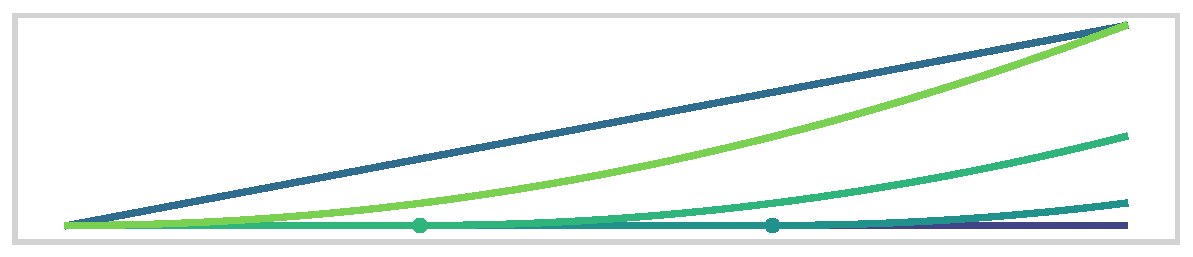
\includegraphics[width=\textwidth]{Images/tpb}
\end{center}
}

\end{frame}


\section{Recap}
%\subsection{Additive Models}

\renewcommand{\biggesteq}{\overbrace{f(\nu_{i})}^{v^T_{i}\xi_1}}
\begin{frame}[b]
\frametitle{Additive Models}

Semiparametric regression:

\begin{minipage}[b][4em][b]{\textwidth}
\begin{overprint}
\begin{align*}
\only<1>{
\hat{y}_i = \inserteqstrut{f(\nu_{i})} + u^T_i \gamma
}
\only<2-3>{
\hat{y}_i = \inserteqstrut{\overbrace{f(\nu_{i})}^{v^T_{i}\xi}} + u^T_i \gamma
}
\only<4-5>{
\hat{y}_i = \overbrace{f_1(\nu_{i1})}^{v^T_{i1}\xi_1} + ... + \overbrace{f_p(\nu_{ip})}^{v^T_{ip}\xi_p} + u^T_i \gamma
}
\end{align*}
\end{overprint}
\vspace{-2.5em}
\end{minipage}

\begin{minipage}[t][0em][t]{\textwidth}
\vspace{-0.5em}
\only<3->{In matrix notation:}
\end{minipage}

\begin{minipage}[b][4em][b]{\textwidth}
\begin{overprint}
\begin{align*}
\only<3>{
\hat{y} = V\xi + U\gamma
}
\only<5>{
\hat{y} = V_1\xi_1 + ... + V_p \xi_p + U\gamma =\sum_{j=1}^p V_j\xi_j + U\gamma
}
\end{align*}
\end{overprint}
\vspace{-3em}
\end{minipage}


\begin{center}
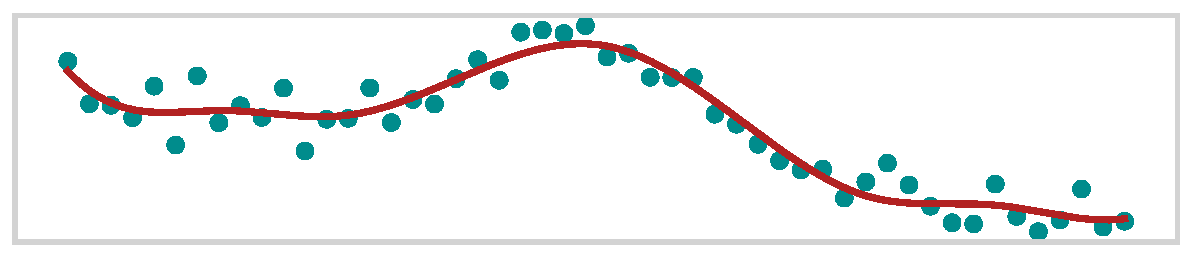
\includegraphics[width=\textwidth]{Images/flex}
\end{center}

\end{frame}


\begin{frame}[b]
\frametitle{Splines}

Spline functions are \textbf{piecewise polynomial segments} (called basis functions) joined together smoothly at so-called knots.
\begin{overprint}
\begin{align*}
\hat{y} = V\xi + U\gamma 
\onslide<2-3>{
= \begin{pmatrix}
b_1(x_1) & \dots & b_k(x_1) \\
 \vdots  & \ddots & \vdots \\
b_1(x_n) & ... & b_k(x_n)
\end{pmatrix} 
\begin{pmatrix}
\xi_1 \\
 \vdots   \\
\xi_k 
\end{pmatrix} 
+ 
\begin{pmatrix}
1 &  x_1 \\
 \vdots & \vdots \\
1 & x_n
\end{pmatrix} 
\begin{pmatrix}
\gamma_1 \\
\gamma_2 
\end{pmatrix} 
}
\end{align*}


\onslide<3>{
\vspace{0.5em}
with basis functions $b_1(.), ..., b_k(.)$, e.\,g.\ \textit{B-spline}, truncated power basis, natural cubic spline, ...
\vspace{-1.5em}
}
\end{overprint}



%B-Spline

\begin{center}
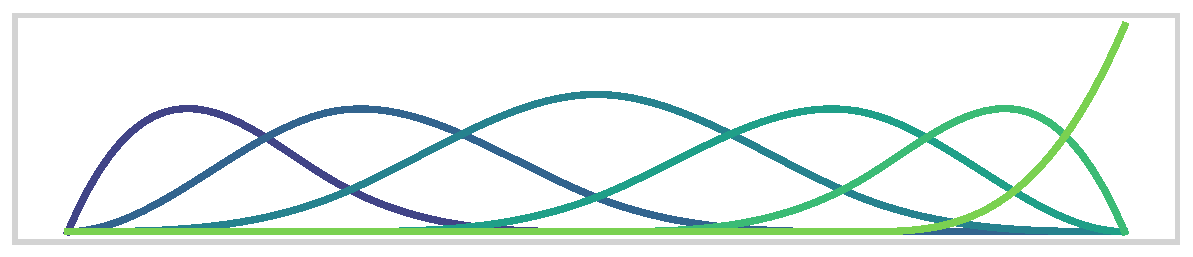
\includegraphics[width=\textwidth]{Images/bases}
\end{center}

\end{frame}

\renewcommand{\biggesteq}{\int\limits_{x_1}^{x_n} \left[ f''(x)\right]^2dx}
\begin{frame}[b]
\frametitle{Roughness Penalty}

Penalized Regression Spline: 

\begin{overprint}
\begin{align*}
\mkern105mu \log L(\xi, \gamma) + \lambda
    \onslide<1>{\inserteqstrut{ \int\limits_{x_1}^{x_n} \left[ f''(x)\right]^2dx}}
    \onslide<2-3>{\inserteqstrut{ \mkern-105mu \xi^T K \xi}}
\end{align*}
\end{overprint}



\begin{minipage}[b][2em][b]{\textwidth}


\begin{overprint}
\begin{flushleft}
\onslide<1>{Control wiggliness (bias-variance tradeoff):}\onslide<2>{\hspace{-17.6em}e.\,g.\ first order differences $\xi^TK\xi = \sum(\xi_{k+1} - \xi_{k})^2$:}\onslide<3>{\hspace{-22.1em} Problem: How to choose $\lambda$?}
\end{flushleft}
\vspace{-2em}
\end{overprint}

\end{minipage}

\begin{center}
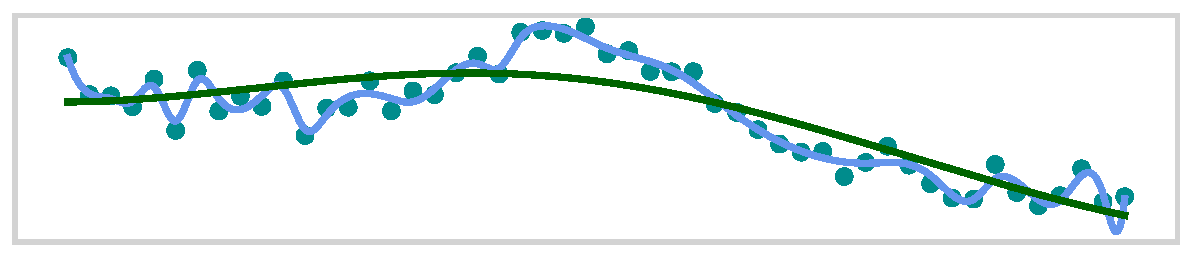
\includegraphics[width=\textwidth]{Images/wiggly}
\end{center}

\end{frame}
%\subsection{Mixed Models}
\begin{frame}
\frametitle{Mixed Models}

\vspace{-1em}

$$y_i = \underbrace{X_i \beta}_{\mathclap{\text{fixed effects}}} + \overbrace{Z_i b_i}^{\mathclap{\text{random effects}}} + \: \epsilon_i$$

\pause

\begin{tabular}{ll}
\textcolor{beamer@postercolour}{\textbf{Classical View}} & random effects reflect that the individuals/  \\
&  clusters are a \textbf{random sample} of a larger  \\
& population (not always appropriate) \vspace{0.5em} \pause \\


\textcolor{beamer@postercolour}{\textbf{Marginal View}} & random effects induce a general linear model \\
&  with \textbf{correlated errors} \vspace{0.5em} \pause \\

\tikzmark{mixed1}{\textcolor{beamer@postercolour}{\textbf{Bayesian View}}}  & the random effects distribution is a \textbf{prior} on \\
& the random effects \vspace{0.5em} \pause \\

\textcolor{beamer@postercolour}{\textbf{Penalization View}} & the random effects distribution results in a \\
& \textbf{penalty} on the random effects leading to \\
& \tikzmark{mixed4}{\textbf{shrinkage}}  \\
\end{tabular}

 \pause\tikz[overlay,remember picture]{\draw[draw=red,thick,double,fill opacity=0.2] ($(mixed1)+(-0.5,0.5)$) rectangle ($(mixed4)+(7.4,-0.3)$);}


				
\end{frame}


\section{Representation}

\begin{frame}
\frametitle{Empirical Bayes}

\begin{itemize}
\item \textcolor{beamer@postercolour}{\textbf{Idea:}} Use Mixed Model inference: $y = \sum_{j=1}^p \underbrace{V_p \xi_p}_{\mathclap{\text{random effects}}} + \overbrace{U \gamma}^{\mathclap{\text{fixed effects}}} + \: \epsilon$ \pause
\vspace{1em}


\textcolor{beamer@postercolour}{Prior: } $ p(\gamma) \propto \text{const.}$ \pause

\textcolor{beamer@postercolour}{Prior: }  $p(\xi_j|\tau_j^2)  \propto \exp\left(-\frac{1}{2\tau^2_j} \xi_j^T\Sigma^{-1}_j \xi_j\right) $  \pause

\textcolor{beamer@postercolour}{Posterior: }
$p(\xi_1, ... \xi_p, \gamma|y) \propto L(y,\xi_1, ... \xi_p, \gamma)\prod_{j=1}^p p(\xi_j|\tau_j^2) $ \pause
\vspace{1em}

\item Maximum Likelihood for $\tau_j^2$ (so far treated as fixed):
$$\max_{\tau_1, ..., \tau_p} \log L(\gamma, \xi_1,...,\xi_p) - \sum_{j=1}^p \underbrace{\frac{1}{2\tau^2_j}}_{\lambda_j} \xi_j^T \underbrace{\Sigma^{-1}_j}_{K_j} \xi_j$$
\end{itemize}

\pause

$\Rightarrow$ Empirical Bayes is equivalent to penalized Maximum Likelihood

%Problem: improper priors therefore reparameterize?

\end{frame}



%\begin{frame}
%\frametitle{Example: Truncated Power Basis}
%
%\begin{align*}
%\begingroup % keep the change local
%\setlength\arraycolsep{3pt}
%y = V\xi + U\gamma 
%\onslide<2-3>{
%= \begin{pmatrix}
%x_1^2 &  (x_1{-}\kappa_1)_+^2 &  (x_1{-}\kappa_2)_+^2 \\
% \vdots  & \vdots & \vdots \\
%x_n^2 & (x_n{-}\kappa_1)_+^2 & (x_n{-}\kappa_2)_+^2
%\end{pmatrix} \!\!
%\begin{pmatrix}
%\xi_1 \\
%\xi_2   \\
%\xi_3 
%\end{pmatrix} 
%\! {+} \!
%\begin{pmatrix}
%1 &  x_1 \\
% \vdots & \vdots \\
%1 & x_n
%\end{pmatrix} \!\!
%\begin{pmatrix}
%\gamma_1 \\
%\gamma_2
%\end{pmatrix} 
%}
%\endgroup
%\end{align*}
%
%$$\log L(\xi, \gamma) + \lambda \xi^T D \xi$$
%
%Problem: $D$ improper
%
%\onslide<1->{
%\begin{center}
%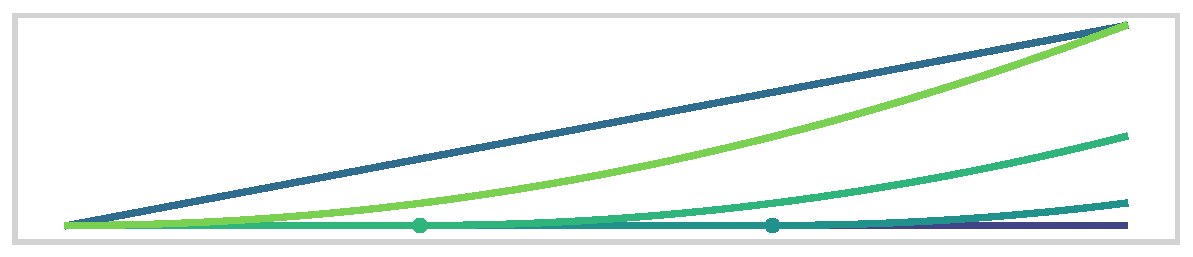
\includegraphics[width=\textwidth]{Images/tpb}
%\end{center}
%}
%
%\end{frame}





\begin{frame}
\frametitle{Mixed Model Representation}
% equivalent to variance components model (components of b_i are independent)

\textcolor{beamer@postercolour}{\textbf{Idea:}} Use Mixed Model inference: $y = \sum_{j=1}^p \underbrace{V_p \xi_p}_{\mathclap{\text{random effects}}} + \overbrace{U \gamma}^{\mathclap{\text{fixed effects}}} + \: \epsilon$

\vspace{1em}




\onslide<2->{
\textcolor{beamer@postercolour}{\textbf{Problem:}} $K_j$ as precision matrix is problematic as $K_j$ is often rank deficient, 
\textcolor{beamer@postercolour}{e.\,g.} $\xi^TK\xi = \sum(\xi_{k+1} - \xi_{k})^2$ $\rightarrow$ $\xi_1$ not penalized:

The Gaussian prior $p(\xi_j|\tau_j^2) \propto \exp\left(-\frac{1}{2\tau^2_j} \xi_j^TK_j \xi_j\right)$ is improper.


\vspace{1.4em}
}



\onslide<3->{
\textcolor{beamer@postercolour}{\textbf{Solution:}} Separate $\xi_j$ into $\xi_j = \tilde{X}_j \beta_j + \tilde{Z}_j b_j$:

\begin{itemize} \pause\pause\pause
\item $\beta$: non-penalized parts with a flat prior 
$\text{dim}(\beta_j) = \text{dim}(\xi_j) {-} \text{rank}(K_j)$  \pause

\item $b$: penalized parts with a proper (Gaussian) prior 

$\text{dim}(b_j) =\text{rank}(K_j)$
\end{itemize}
\vspace{-1em}
}


\end{frame}

%\begin{frame}
%\frametitle{...}

%Graphical: $\beta_j$ captures non-penalized part, $b_j$ captures the orthogonal %deviation from the unpenalized part.
%\end{frame}



\begin{frame}[t]
\frametitle{Mixed Model Representation}

\only<1>{
\begin{center}
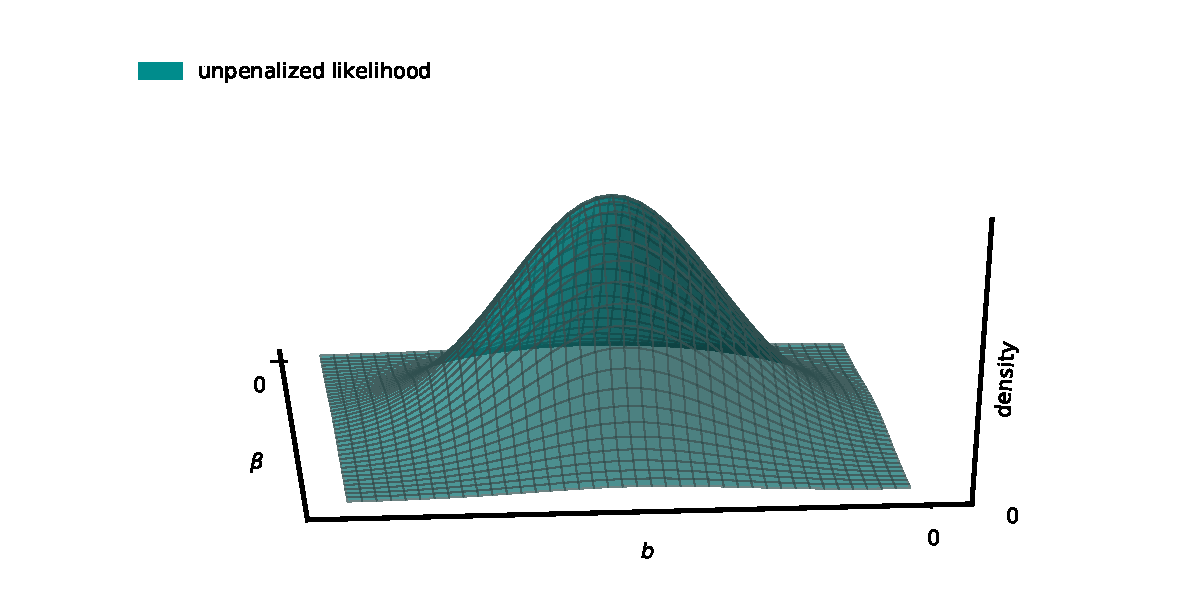
\includegraphics[width=\textwidth, trim={1.8cm 0.5cm 1.8cm 1cm},clip]{Images/priorispenalty1}
\end{center}
}

\only<2>{
\begin{center}
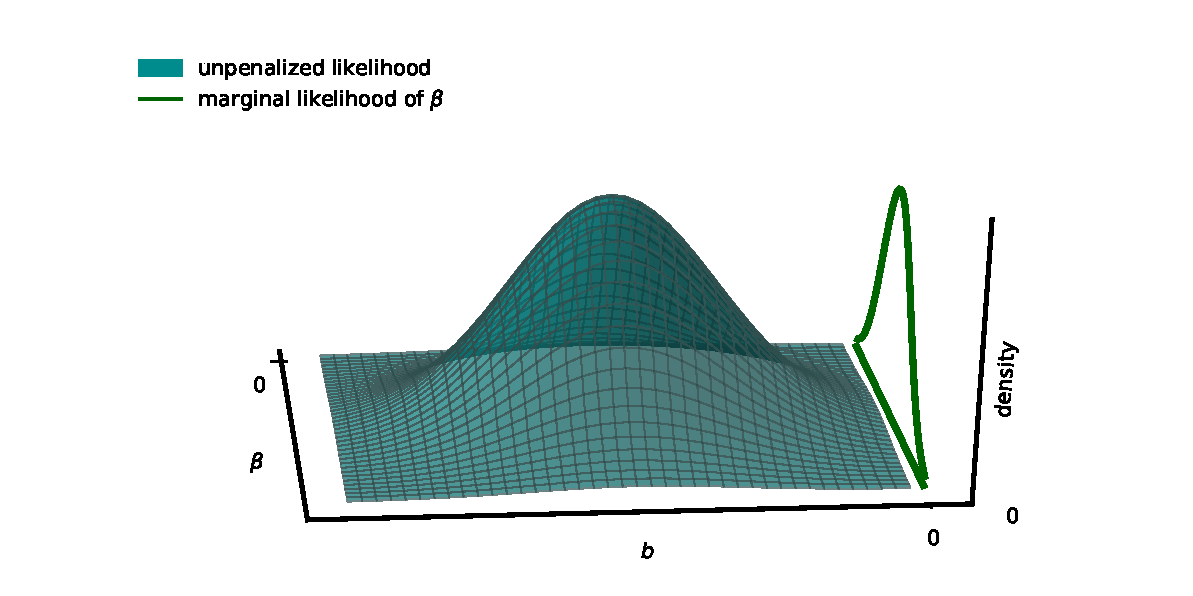
\includegraphics[width=\textwidth, trim={1.8cm 0.5cm 1.8cm 1cm},clip]{Images/priorispenalty2}
\end{center}
}

\only<3>{
\begin{center}
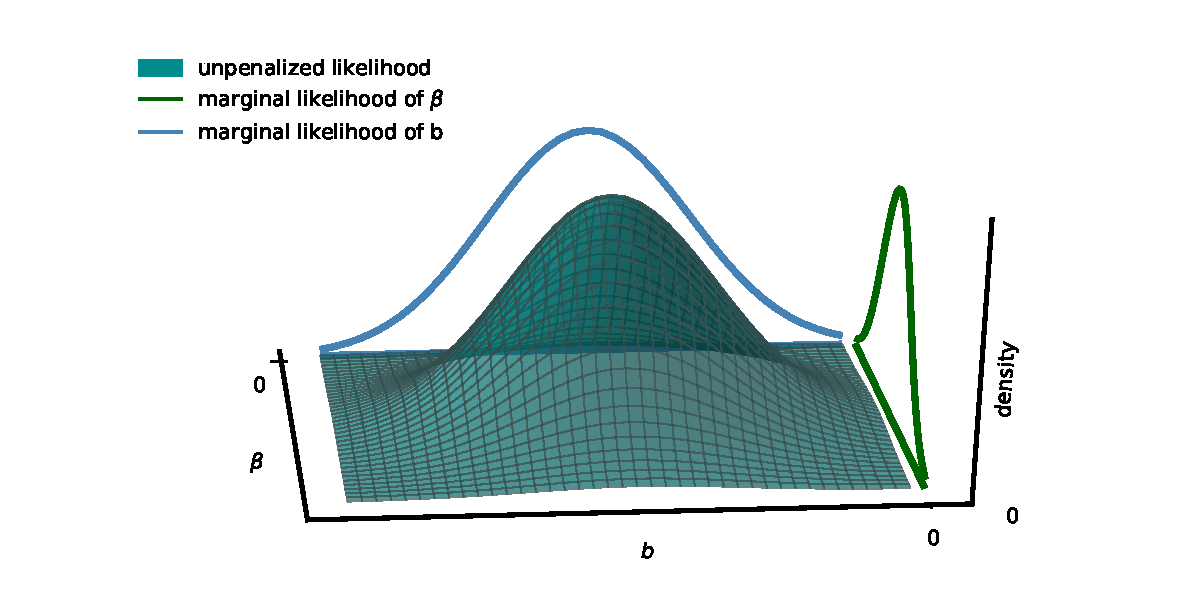
\includegraphics[width=\textwidth, trim={1.8cm 0.5cm 1.8cm 1cm},clip]{Images/priorispenalty3}
\end{center}
}

\only<4>{
\begin{center}
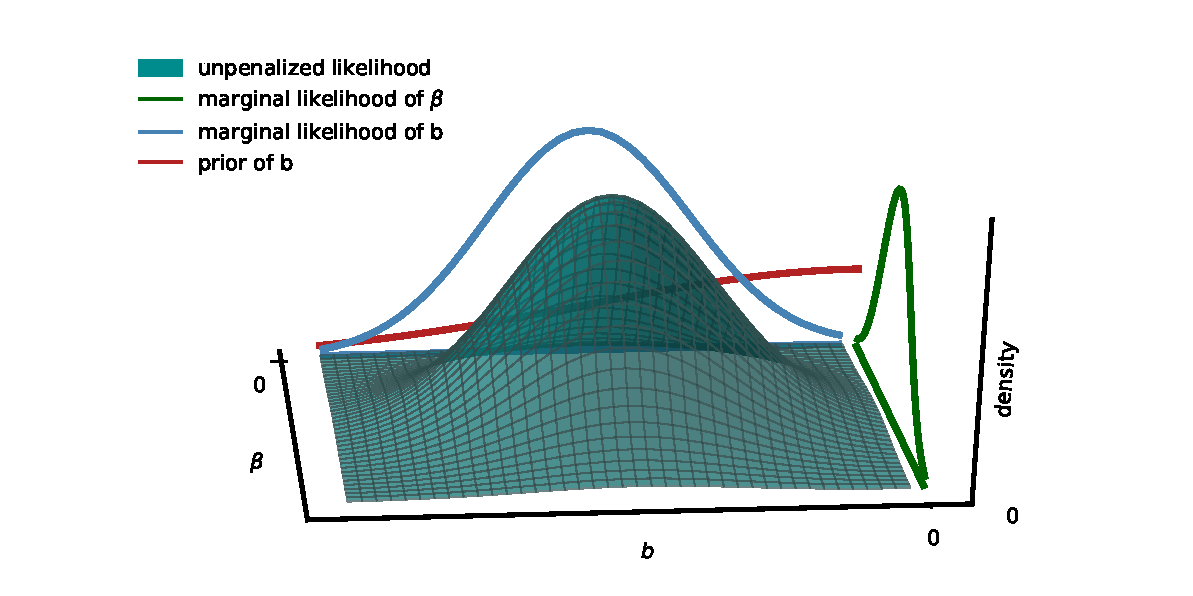
\includegraphics[width=\textwidth, trim={1.8cm 0.5cm 1.8cm 1cm},clip]{Images/priorispenalty4}
\end{center}
}

\only<5>{
\begin{center}
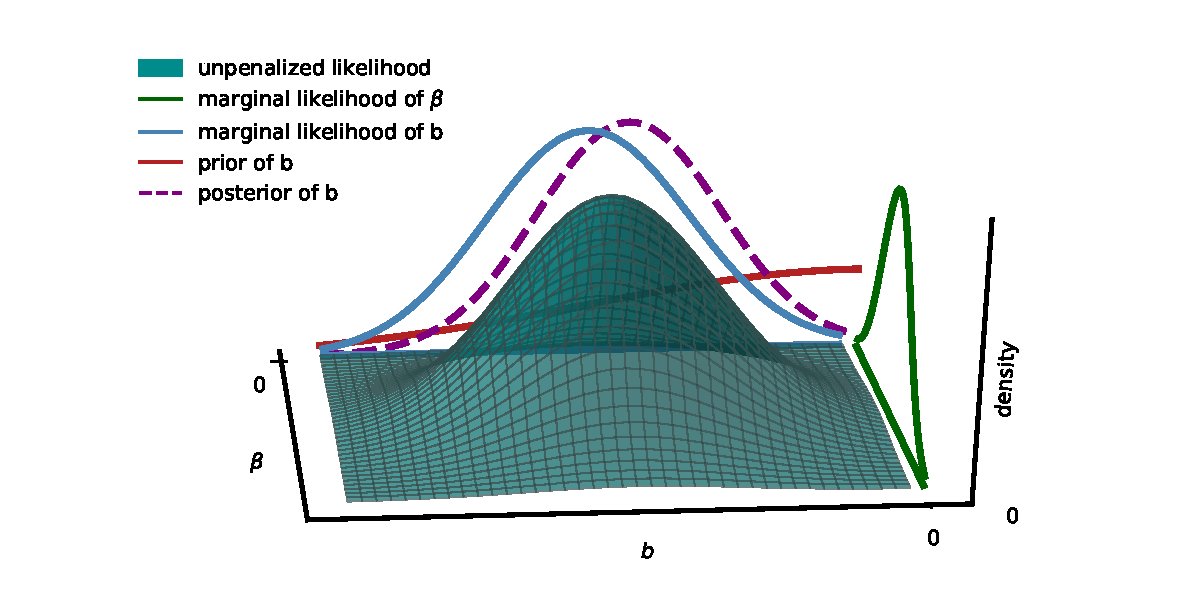
\includegraphics[width=\textwidth, trim={1.8cm 0.5cm 1.8cm 1cm},clip]{Images/priorispenalty5}
\end{center}
}

\only<6-7>{
\begin{center}
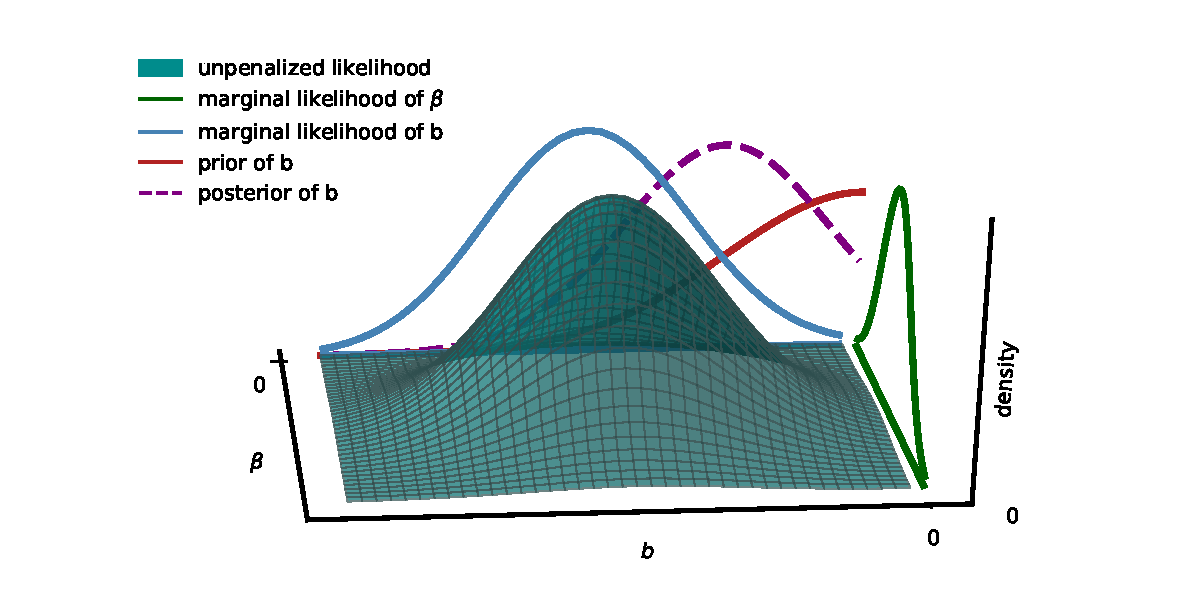
\includegraphics[width=\textwidth, trim={1.8cm 0.5cm 1.8cm 1cm},clip]{Images/priorispenalty6}
\end{center}

\only<7>{The lower the prior variance, the higher the penalty!}
}


\end{frame}

\renewcommand{\biggesteq}{\overbrace{(\tilde{X}_j \beta_j + \tilde{Z}_j b_j)}^{\xi_j} + U\gamma =   X\beta + Zb}
\begin{frame}
\frametitle{Mixed Model Representation}

\begin{columns}[T]
\begin{column}{0.58\textwidth}
\textcolor{beamer@postercolour}{Decomposition $\xi_j = \tilde{X}_j \beta_j + \tilde{Z}_j b_j$:}  

\begin{minipage}[t][5em][t]{\textwidth}
\vspace{-1em}
\begin{overprint}
\begin{align*}
y = \sum_{j=1}^p V_j
\only<1>{
\inserteqstrut{ \xi_j + U\gamma }
}
\only<2>{
\inserteqstrut{\overbrace{(\tilde{X}_j \beta_j + \tilde{Z}_j b_j)}^{\xi_j} + U\gamma }
}
\only<3->{
\inserteqstrut{\overbrace{(\tilde{X}_j \beta_j + \tilde{Z}_j b_j)}^{\xi_j} + U\gamma =   X\beta + Zb } 
}
\end{align*}
\end{overprint}
\vspace{-1em}
\end{minipage}



\end{column}
\begin{column}{0.33\textwidth}
\vspace{-0.5em}
\only<3->{
\begin{align*}
\beta &:= (\beta_1^T,..., \beta_p^T, \gamma^T) \\
b &:= (b_1^T,...,b_p^T) \\
Z &:= V_j \tilde{Z}_j \\
X &:= (V_j \tilde{X}_j, U)
\end{align*}
}
\end{column}
\end{columns}

\onslide<4->{
\textcolor{beamer@postercolour}{Requirements:}

\begin{enumerate}
\item<5-> 1-on-1 transformation: matrix $(\tilde{X}_j \:\:  \tilde{Z}_j)$ has full rank 
\item<6-> $\tilde{X}_j$ and $\tilde{Z}_j$ are orthogonal: $\tilde{X}_j^T \tilde{Z}_j = 0$
\item<7-> $\beta_j$ not penalized by $K_j$: $\tilde{X}_j^T K_j \tilde{X}_j = 0$
\item<8-> Gaussian prior for $b_j$: $\tilde{Z}_j^T K_j \tilde{Z}_j = I_{kj}$
\end{enumerate}
}


\end{frame}




\begin{frame}
\frametitle{Mixed Model Representation}

\textcolor{beamer@postercolour}{log-Prior: } 

\begin{minipage}[t][4em][t]{\textwidth}
\vspace{-1em}
\begin{overprint}
\begin{align*}
\log p(\xi_j|\tau_j^2)  \propto -\frac{1}{2\tau^2_j} \xi_j^TK_j \xi_j
\onslide<2->{ = -\frac{1}{2\tau_j^2} b_j^T b_j
}
\end{align*}
\end{overprint}
\vspace{-3em}
\end{minipage}

\begin{minipage}[t][10em][t]{\textwidth}
\only<3->{$\Rightarrow p(\beta) \propto \text{const.}$}

\only<4->{$\Rightarrow p(b_j) \sim N(0,\tau_j^2I_{kj})$}

\vspace{2em}

\only<5->{
\textcolor{beamer@postercolour}{log-Posterior: } $$l_p(\beta,b|y) = l(y,\beta,b) - \sum_{j=1}^p \overbrace{\frac{1}{2\tau_j^2}}^{=\lambda} b_j^T  b_j $$
}
\end{minipage}

\end{frame}

\section{Inference}

\begin{frame}
\frametitle{Estimates $\hat{\beta}$ and $\hat{b}$}
In order to maximize the (log-)Posterior (equivalent to ML), derive estimates for $\beta$ and $b$ simultaneously based on known $\sigma^2$ and $\tau^2$.
\vspace{2em}

\onslide<2->{
\textcolor{beamer@postercolour}{Mixed Model equations:}
$$\overbrace{\begin{pmatrix}
X^TWX & X^TWZ \\
Z^TWX & Z^TWZ + Q^{-1}
\end{pmatrix}}^{\text{Fisher information}}
\begin{pmatrix}
\hat{\beta} \\
\hat{b}
\end{pmatrix} =
\begin{pmatrix}
X^TWy \\
Z^TWy
\end{pmatrix}$$

 with $W=\text{diag}(\sigma^2)$ and $Q=\text{blockdiag}(\tau_1^2I_{k1},..., \tau_p^2I_{kp})$
}

\end{frame}

\begin{frame}
\frametitle{Variance Estimates}

\textcolor{beamer@postercolour}{Maximum Likelihood (integrate $b$ out)} 

\begin{itemize}
\item uses (partialy) marginal distribution $y \sim \mathrm{N}(X\beta,\Sigma)$

\begin{enumerate}
\item Derive $\hat{\beta}$ analytically
\item Plug in to get profile likelihood for $\tau^2$ and $\sigma^2$
\item Maximize numerically
\end{enumerate}

\item estimates variance components of posterior mode
\end{itemize}

\vspace{1em}
\pause

\textcolor{beamer@postercolour}{Restricted ML integrate ($b$ and $\beta$ out)}

\begin{itemize}
\item directly uses marginal distribution of $y$

\item Advantages over ML:
\begin{itemize}
\item[$+$] considers loss of degrees of freedom due to estimation of $\beta$ 
\item[$+$] estimates mode of the marginal posterior for the variances
\end{itemize}
\end{itemize}


\end{frame}

\begin{frame}
\frametitle{Variance Estimates $\hat{\sigma}^2$ and $\hat{\tau}^2$}

Maximize the restricted likelihood (REML) using Newton-Raphson:
\begin{center}
\only<1>{
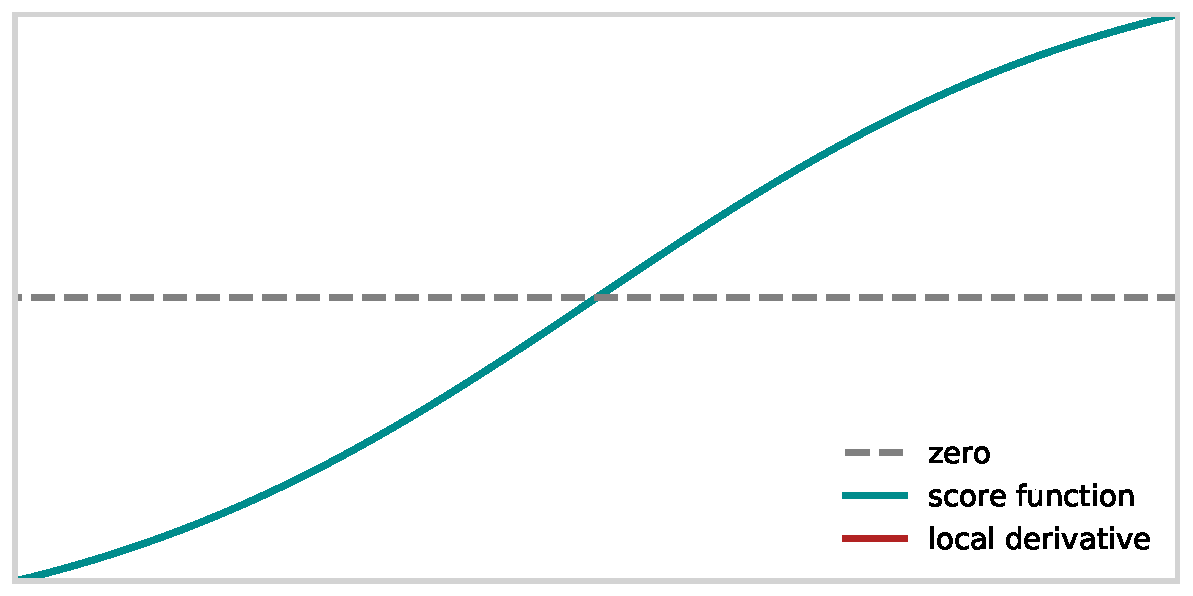
\includegraphics[width=\textwidth]{Images/newton}
}
\only<2>{
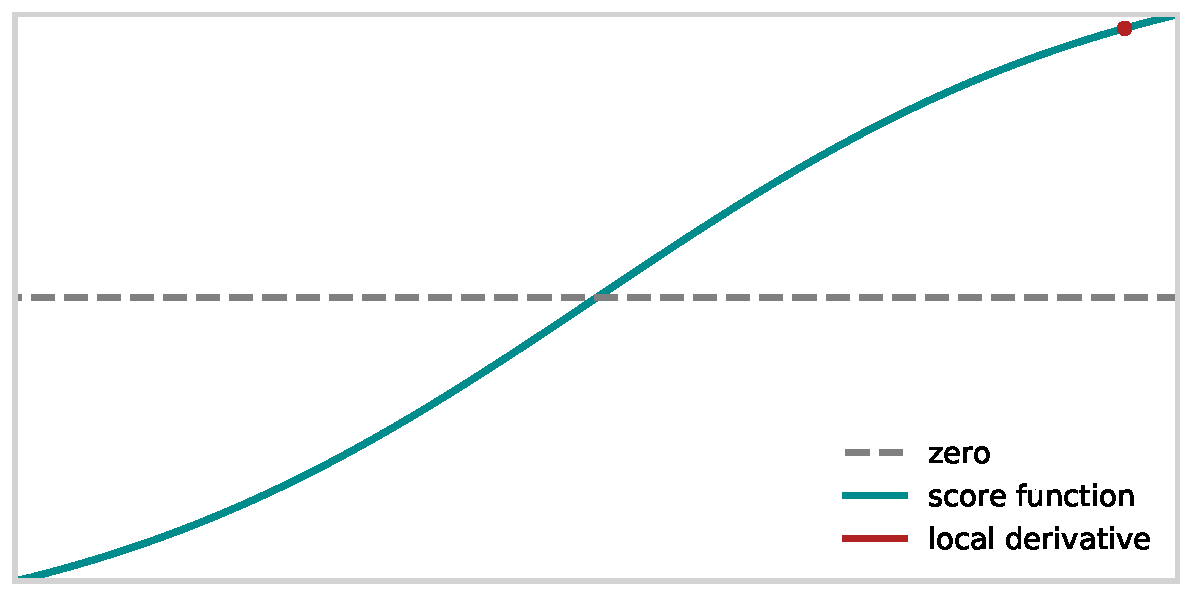
\includegraphics[width=\textwidth]{Images/newton_scatter0}
}
\only<3>{
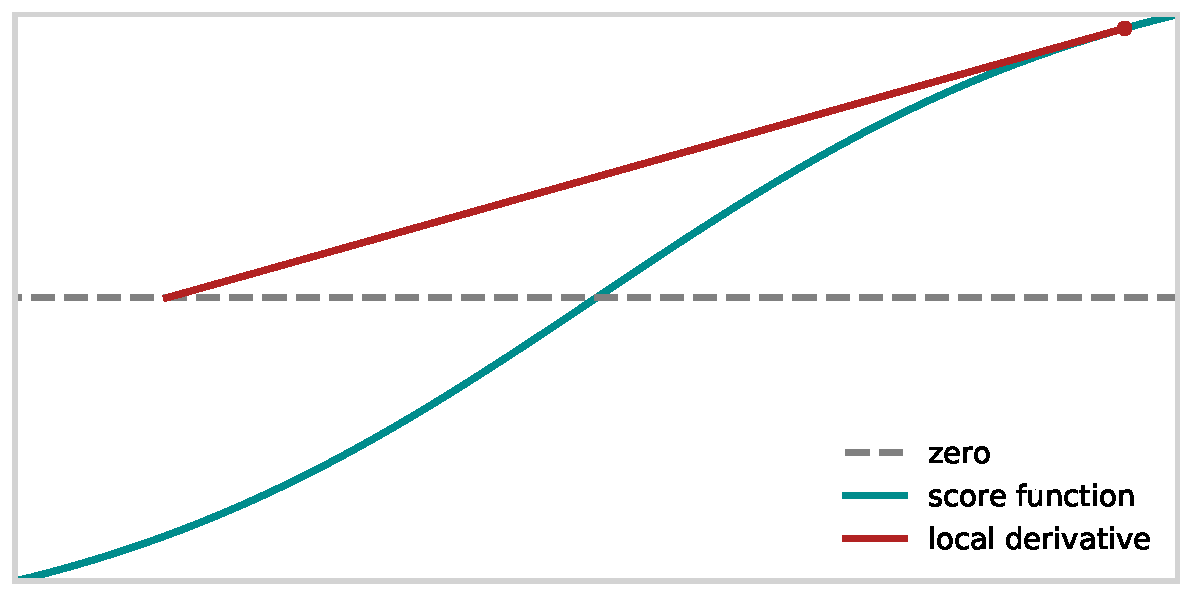
\includegraphics[width=\textwidth]{Images/newton_line0}
}
\only<4>{
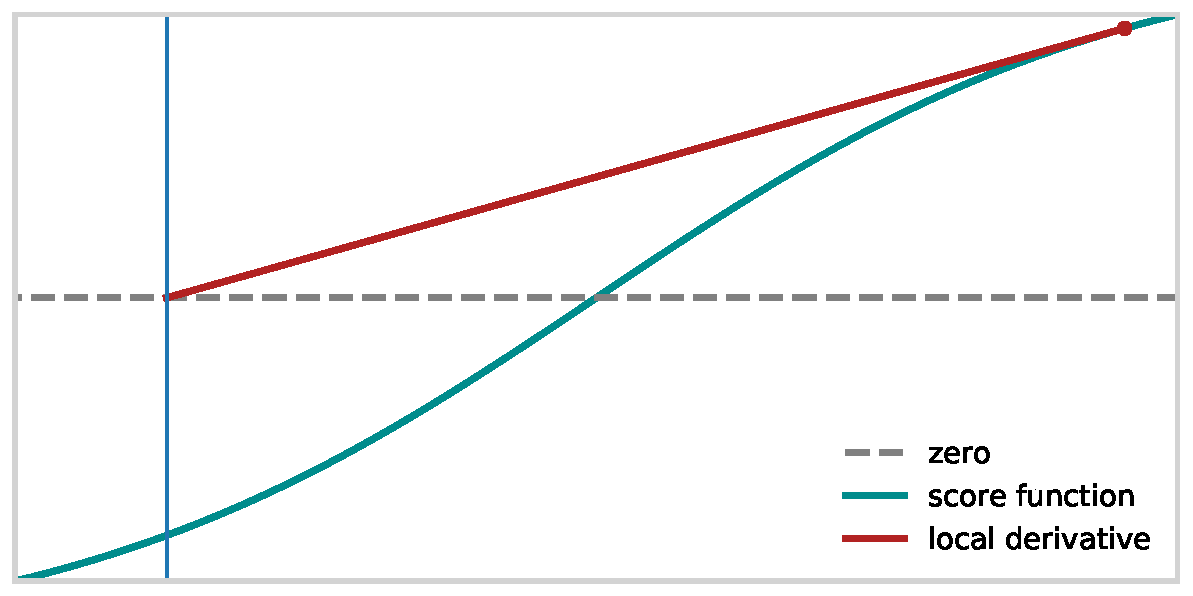
\includegraphics[width=\textwidth]{Images/newton_point0}
}
\only<5>{
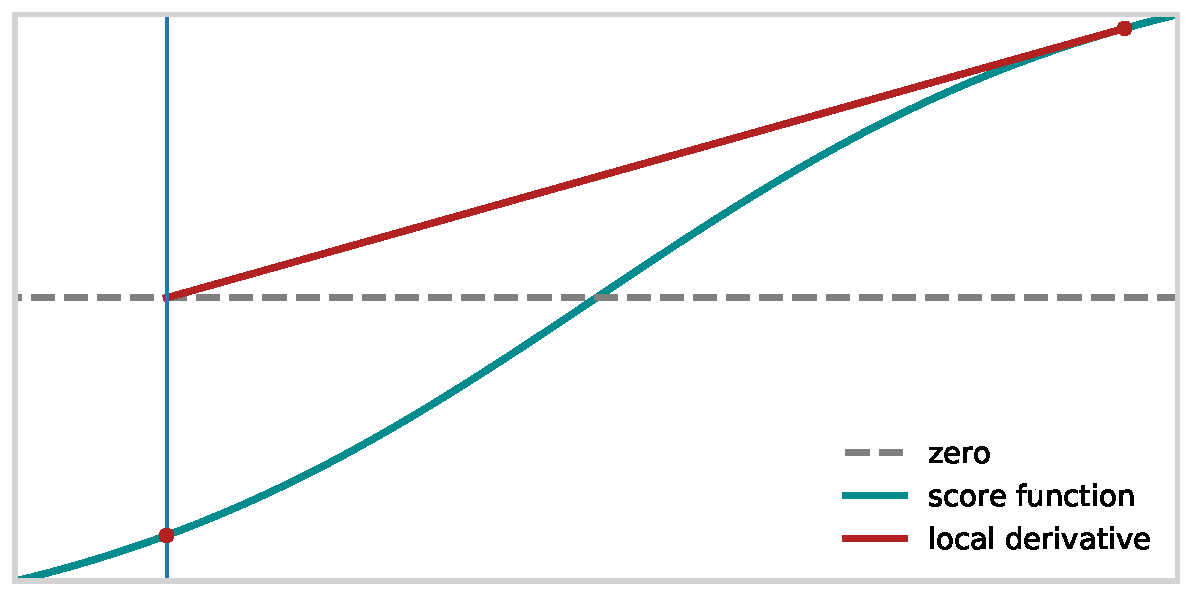
\includegraphics[width=\textwidth]{Images/newton_scatter1}
}
\only<6>{
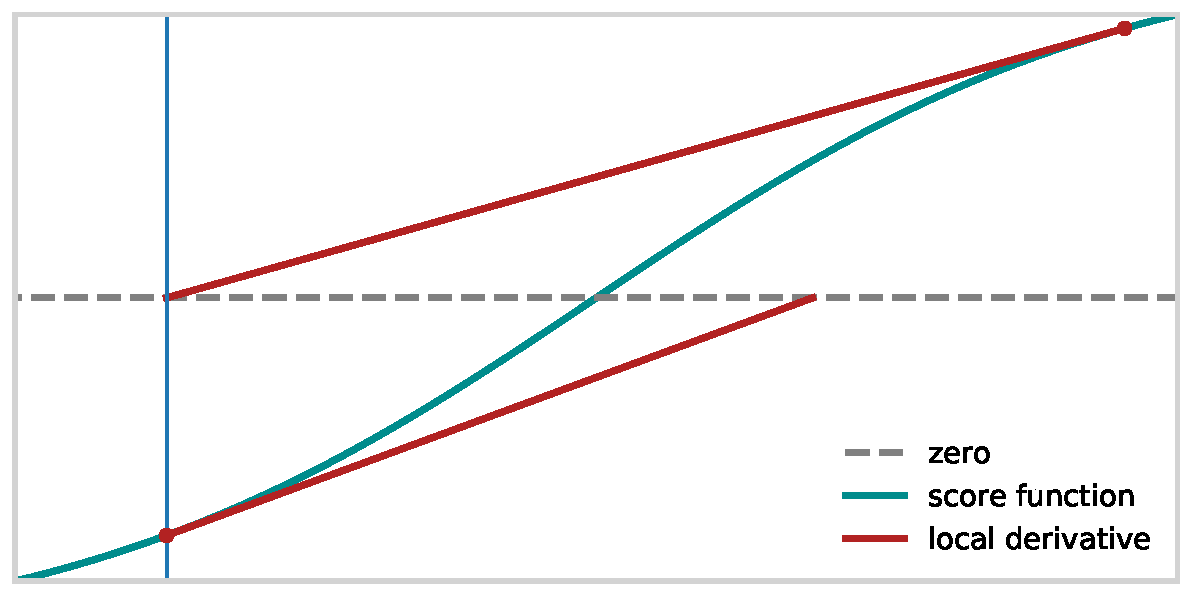
\includegraphics[width=\textwidth]{Images/newton_line1}
}
\only<7>{
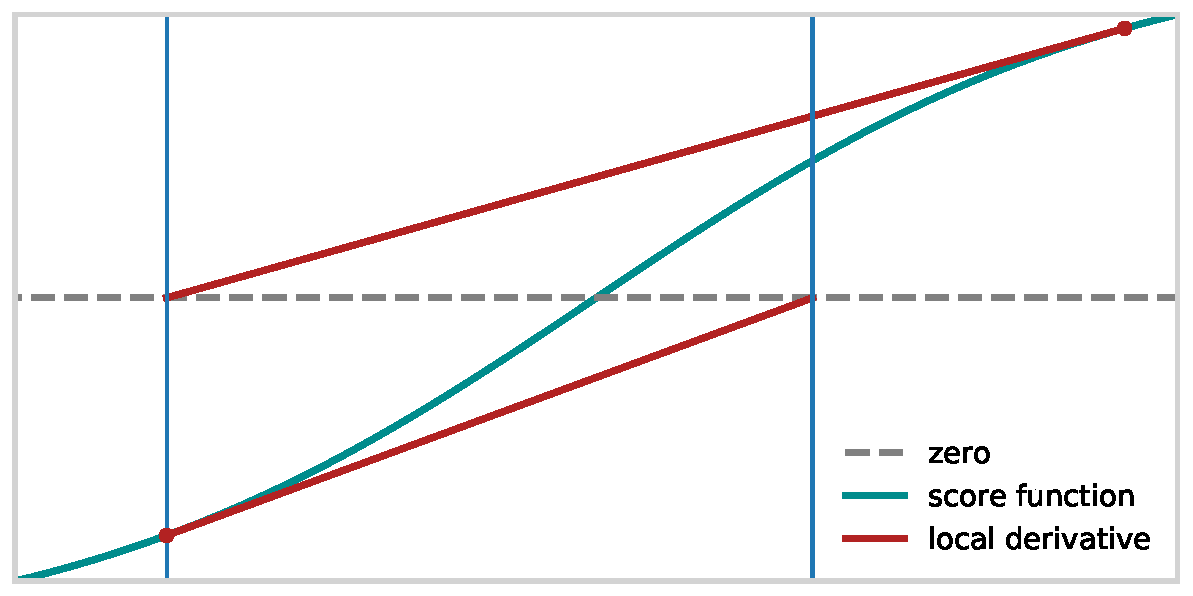
\includegraphics[width=\textwidth]{Images/newton_point1}
}
\only<8>{
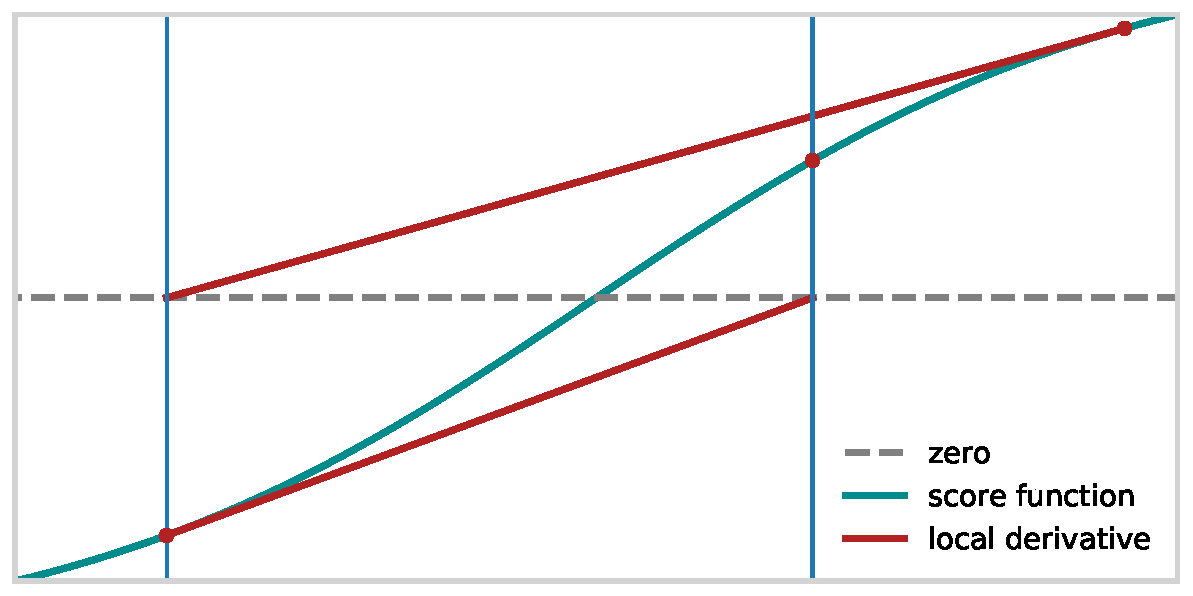
\includegraphics[width=\textwidth]{Images/newton_scatter2}
}
\only<9>{
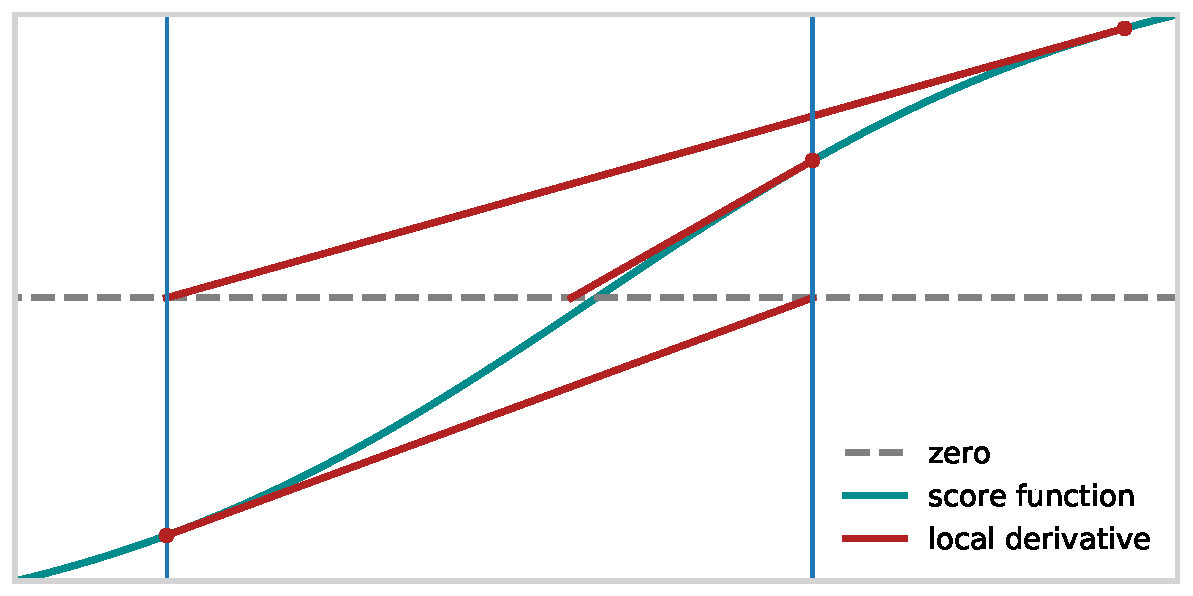
\includegraphics[width=\textwidth]{Images/newton_line2}
}
\only<10>{
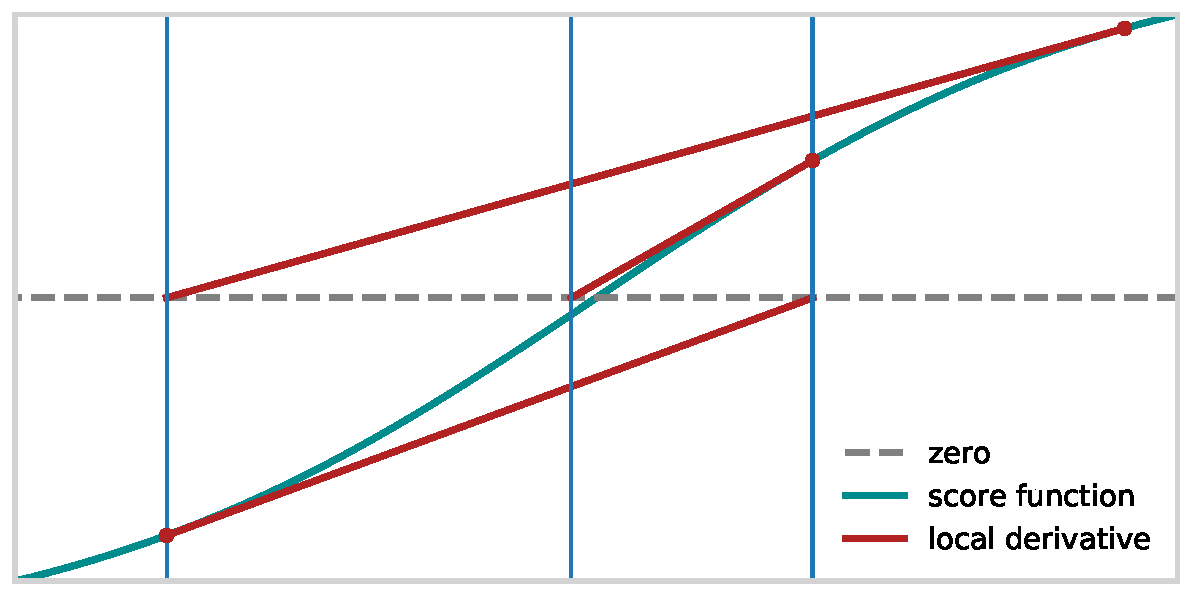
\includegraphics[width=\textwidth]{Images/newton_point2}
}
\only<11>{
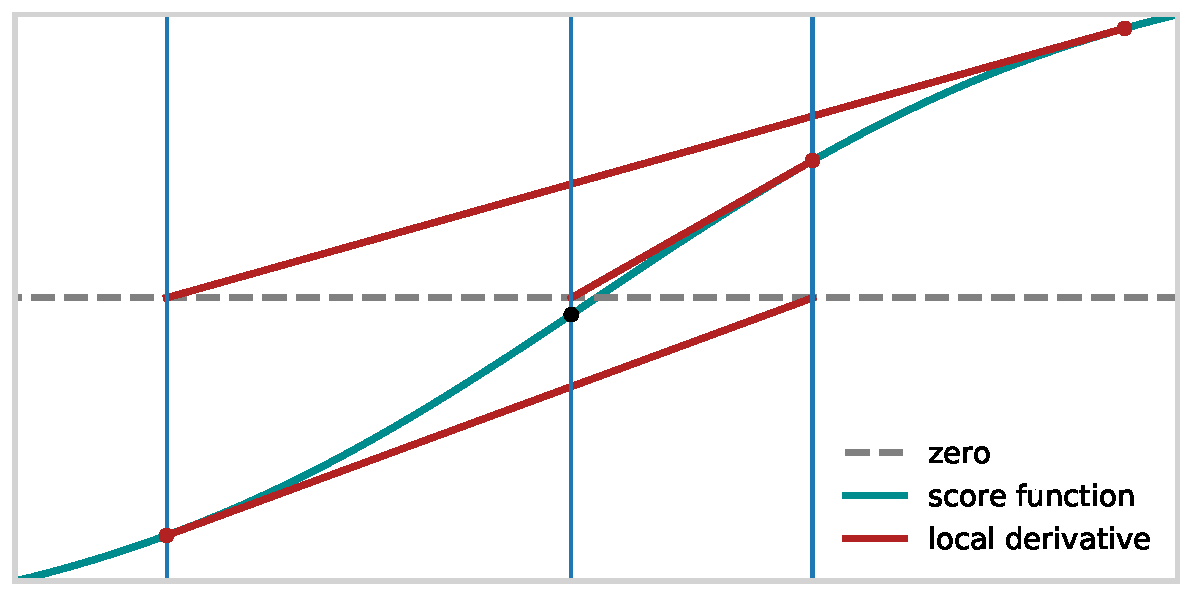
\includegraphics[width=\textwidth]{Images/newton_finished}
}


\end{center}

\end{frame}




%\begin{frame}
%\frametitle{Variance Estimates}
%$$l(y,\beta,b) \approx \sum_{i=1}^n \frac{(y_i-\mu_i)^2}{w_iv(\mu_i)/\phi} = (y-\mu)^TS^{-1}(y-\mu)$$
%
%Approximation by Pearson's $\chi^2$-statistic is equivalent to the Laplace approximation
%
%With working observations $\tilde{y}$ we have $(y-\mu) = D(\tilde{y}-X\beta-Zb)$ and
%
%\begin{align*}
%l(y,\beta,b) &\approx (\tilde{y}-X\beta-Zb)^TD^TS^{-1}D(\tilde{y}-X\beta-Zb)\\
%&= (\tilde{y}-X\beta-Zb)^TW(\tilde{y}-X\beta-Zb)
%\end{align*}
%
%ignoring the dependence of $W$ on the variance parameters:
%
%$$\tilde{y}|\beta,b \overset{a}{\sim} \mathrm{N}(X\beta+Zb,w^{-1})$$
%
%
%\end{frame}



%\section{Choosing $\lambda$} %Chapter 7 more on choosing the smoothing criterion, why is choosing lambda the same as choosing the prior variance





\begin{frame}
\frametitle{(RE)ML estimation}

\textcolor{beamer@postercolour}{\textbf{Single iterations (old)}}
\begin{enumerate}
\item Update  $\hat{\beta}$ and $\hat{b}$ given the current $\lambda$
\item Update $\hat{\lambda}$ using Fisher-Scoring (or Newton-Raphson)
\item Iterate until convergence
\end{enumerate}

\vspace{0.5em}
\pause

\textcolor{beamer@postercolour}{\textbf{Nested iterations (new)}}
\begin{enumerate}
\item \textbf{Estimate the penalty $\lambda$:}

Using Newton-Raphson
\begin{itemize}
\item For each $\hat{\lambda}$: Get estimates for $\beta$ and $b$: 

Solve with penalized iteratively re-weighted least squares (PIRLS) and Newton-Raphson
\end{itemize}
\item \textbf{Iterate until convergence}
\end{enumerate}
\end{frame}





\section{Conclusion}


\begin{frame}
\frametitle{Comparison of Mixed Model Approach}
\begin{columns}[T]
\begin{column}{0.5\textwidth}
\centering{\textcolor{beamer@postercolour}{Fully Bayesian approach \\(MCMC)}}
\begin{itemize}
\item[$+$] no reparameterization needed
\item[$-$] identifiability problems less detectable
\item[$-$] how to choose hyperpriors?
\item[$-$] Markov chain convergence is difficult to determine
\end{itemize}
\end{column}
\begin{column}{0.5\textwidth}
\centering{\textcolor{beamer@postercolour}{Prediction error methods \\ (AIC, GCV)}}
\begin{itemize}
\item[$+$] better prediction error performance 
\item[$-$] worse resistance to overfit
\item[$-$] higher smoothing parameter variability
\item[$-$] increased tendency to multiple minima
\item[$\rightarrow$] \textit{more on that next week}
\end{itemize}
\end{column}
\end{columns}
\end{frame}


%\begin{frame}
%\frametitle{Prospect: GLM}

%GLM



%\end{frame}

\begin{frame}
\frametitle{Summary}

\begin{itemize}
\item Semiparametric models can be \textbf{written as mixed models}.
\item In order to get a proper random effects distribution, the flexible parameters have to be \textbf{separated} into sets of parameters with \textbf{flat priors} and sets with \textbf{proper priors}.
\item The penalty term  is proportional to the inverse of the prior variance: $\mathbf{\boldsymbol{\lambda} \boldsymbol{\propto} \frac{1}{\boldsymbol{\tau}^2}}$
\item For good results in mixed model inference, the \textbf{penalty term} has to be estimated in a \textbf{nested iteration} setup with the other parameters.
\end{itemize}

\end{frame}


\appendix
\begin{frame}
\frametitle{References}
				\begin{thebibliography}{10}
				
\bibitem[Fahrmeir et al., 2013]{fahrmeir}
Fahrmeir, L., Kneib, T., Lang, S., \&  Marx, B. (2006). {\em Regression -- Models, Methods and Applications}.
\newblock Springer-Verlag Berlin Heidelberg.

\bibitem[Kneib, 2006]{kneib}
Kneib, T. (2006). {\em Doctoral Thesis}, LMU Munich.
\newblock Mixed model based inference in structured additive regression.

\bibitem[Wood, 2017]{woodbook}
Wood, S. N. (2017). \\ {\em Generalized Additive Models: An Introduction with R}.
\newblock Chapman and Hall/CRC.

\bibitem[Wood, 2011]{woodpaper}
Wood, S. N. (2011). {\em J.\ R.\ Statist.\ Soc.\ B}, 73: 3--36.
\newblock Fast stable REML and ML estimation of semiparametric GLMs.

\end{thebibliography}
\end{frame}



\begin{frame}
\frametitle{Choosing $\tilde{X}_j$ and $\tilde{Z}_j$ for Mixed Model Representation}

\begin{block}{\small Recap: Conditions}
\small
\begin{enumerate}
\itemsep0em 
\item 1-on-1 transformation: matrix $(\tilde{X}_j \:\:  \tilde{Z}_j)$ has full rank
\item $\tilde{X}_j$ and $\tilde{Z}_j$ are orthogonal: $\tilde{X}_j^T \tilde{Z}_j = 0$
\item $\beta_j$ not penalized by $K_j$: $\tilde{X}_j^T K_j \tilde{X}_j = 0$
\item Gaussian prior for $b_j$: $\tilde{Z}_j^T K_j \tilde{Z}_j = I_{kj}$
\end{enumerate}
\end{block}
\vspace{-1em}
\begin{block}{Setup}
\begin{itemize}
\item $\tilde{X}_j$ is a basis of the null space of $K_j$ (condition 3)
\item $\tilde{Z}_j =L_j (L_j^T L_j)^{-1}$ with $K_j =L_j L_j^T$ (conditions 1 and 4)
\item Choose $L_j$ s.\,t.\ $L_j^T\tilde{X}_j = 0$ and $\tilde{X}_jL_j^T = 0$ (condition 2)

e.\,g.\ spectral decomposition: 
$K_j = \Gamma_j \Lambda_j \Gamma^T$, so $L_j = \Gamma \Lambda_j^{1/2}$
\end{itemize}
\end{block}

\end{frame}



%\begin{frame}
%\frametitle{Smoothing Parameter Selection}
%\begin{columns}[T]
%\begin{column}{0.5\textwidth}
%\centering{\textcolor{beamer@postercolour}{Prediction Error Methods}}
%\begin{itemize}
%\item Examples:
%\begin{itemize}
%\item[*] AIC
%\item[*] GCV
%\end{itemize}
%\item[$+$] Better prediction error performance 
%\item[$-$] weak penalization of overfit: lower convergence of smoothing parameters
%\end{itemize}
%\end{column}
%\begin{column}{0.5\textwidth}
%\centering{\textcolor{beamer@postercolour}{Likelihood Methods}} 
%\begin{itemize}
%\item using mixed models
%\item[$+$] Greater resistance to overfit
%\item[$-$] computationally less reliable
%\begin{itemize}
%\item single iteration methods: might not converge
%\item nested iteration methods: computationally complex
%\end{itemize}
%\item[$\rightarrow$] efficient and stable nested method now available
%\end{itemize}
%\end{column}
%\end{columns}
%
%\end{frame}

%\begin{frame}
%\frametitle{Estimates for $\beta$ and $b$}
%
% Fisher-Scoring for $\beta$ and $b$ (as in GLM):
% \begin{itemize}
%
%\item Score-Function: $s(\beta, b) %= \frac{\partial l_p(\beta,b|y)}{\partial (\beta,b)}
% = \left(\substack{s_\beta(\beta,b) \\ s_b(\beta,b)}\right) = \left(\substack{X^TDS^{-1}(y-\mu) \\ Z^TDS^{-1}(y-\mu)-Q^{-1}b}\right)$
%
%with $D=\text{diag}\left(\frac{\partial h(\eta_i)}{\partial \eta}\right)$ and $S = \text{diag}(\sigma^2_i)$ 
%\item Fisher-Information: $F(\beta,b) = \left(\substack{F_{\beta\beta}(\beta,b) \:\: F_{\beta b}(\beta,b) \\ F_{b\beta}(\beta,b) \:\: F_{bb}(\beta,b)}\right)$
%
%with $F_{\beta\beta}(\beta,b)=X^TDS^{-1}DX$, $F_{\beta b}(\beta,b) =  F_{b\beta}(\beta,b)^T =X^TDS^{-1}DZ$, and $F_{bb}(\beta,b) = Z^TDS^{-1}DZ + Q^{-1}$
%
%\item Estimates: $$\left(\substack{\hat{\beta}^{(k+1)} \\ \hat{b}^{(k+1)}}\right) = \left(\substack{\hat{\beta}^{(k)} \\ \hat{b}^{(k)}}\right) + \left(F^{(k)}\right)^{-1}s^{(k)}$$
%\end{itemize}
%
%\end{frame}


\end{document}
